\documentclass{article} % This command is used to set the type of document you are working on such as an article, book, or presenation

\usepackage{geometry} % This package allows the editing of the page layout
\usepackage{amsmath}  % This package allows the use of a large range of mathematical formula, commands, and symbols
\usepackage{graphicx}  % This package allows the importing of images

\newcommand{\question}[2][]{\begin{flushleft}\textbf{Question #1}: \textit{#2}\end{flushleft}}
\newcommand{\sol}{\textbf{Solution}:} %Use if you want a boldface solution line
\newcommand{\maketitletwo}[2][]{\begin{center}
        \Large{\textbf{Homework 2 Report}
        
            Reinforcement Learning} % Name of course here
        \vspace{5pt}
        
        \normalsize{
            Name: Kai-Jie Lin 
            
            Student ID: 110652019
            
            \today}
        \vspace{15pt}
        \end{center}}
\begin{document}
    \maketitletwo[5]  % Optional argument is assignment number
    %Keep a blank space between maketitletwo and \question[1]
    \section{Implementation}
    \section{Experiment}
    \subsection{Pendulum-v1}
    Training result of DDPG. \\
    Hyperparameters: Learning rate = 0.001, decay rate of learning rate = 0.9, discounted factor = 0.999. \\
    %\begin{table}[h]
    %    \centering
    %    \begin{tabular}{|c|c|c|c|}
    %    \hline
    %    \textbf{Learning Rate(Actor)} & \textbf{Learning Rate(Critic)} & \textbf{Batch Size} \\ \hline
    %    0.0065 & 0.8104 & 0.9700 \\ \hline
    %    \end{tabular}
    %    \caption{Hyperparameters of DDPG}
    %    \label{tab:ddpg_results}
    %\end{table}
    Environment: Pendulum-v1.\\
    Result(EWMA reward): Reach well policy in near 300 steps.\\
    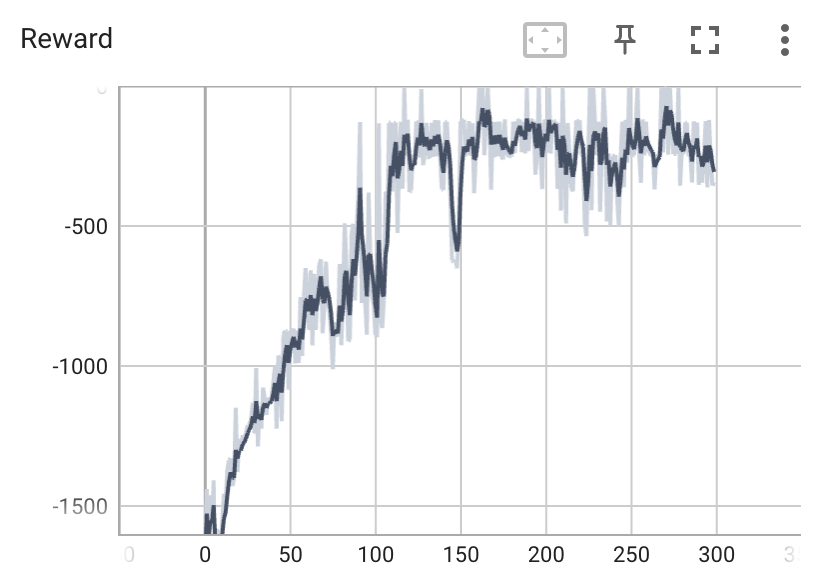
\includegraphics[width=10cm]{./imgs/pendulum/rw.png}
    
\end{document}